\section{Метод №3}\label{meth3}

\subsection{Идея}\label{math3:idea}

\begin{itemize}
	\item[1)] Проводим прямые через точки множеств в направлениях проектирования и получаем множество скрещивающихся прямых.
	\item[2)] Рассматривая искомую прямую как вектор, приложенный к точке, фиксируем точку и составляем функционал суммы квадратов расстояний от проекций прямой до соответствующих множеств точек и минимизируем его (получаем линейную систему).
	\item[3)] Аналогично рассматривая искомую прямую как вектор, приложенный к точке, теперь фиксируем вектор и составляем функционал суммы квадратов расстояний от проекций прямой до соответствующих множеств точек и минимизируем его (тоже получаем линейную систему).
	\item[4)] Некоторыми последовательными изменениями одного параметра при фиксированном другом и наоборот (вектор и точка), минимизируем полученные функционалы и минимизируем отклонение.
\end{itemize}

\begin{center}
	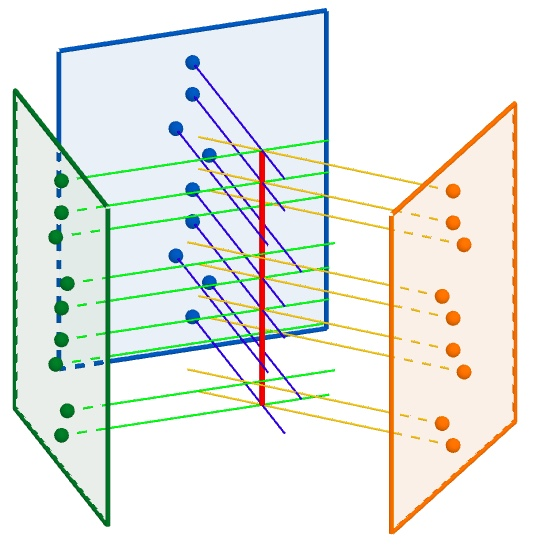
\includegraphics[scale=0.6]{131}

	Рис. 2.4: Построение скрещивающихся прямых через точки множеств.
\end{center}

\begin{center}
	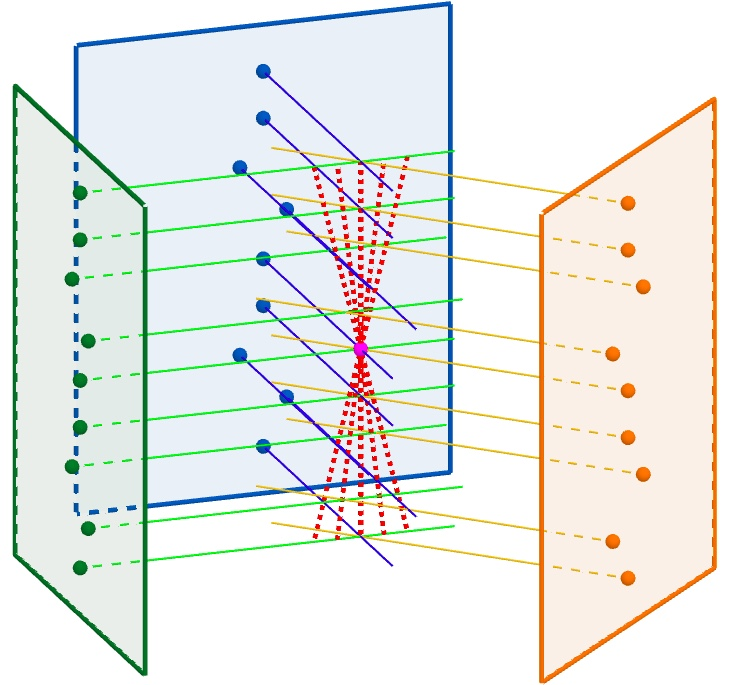
\includegraphics[scale=0.48]{132}

	Рис. 2.5: Изменение вектора прямой при фиксированной точке.

	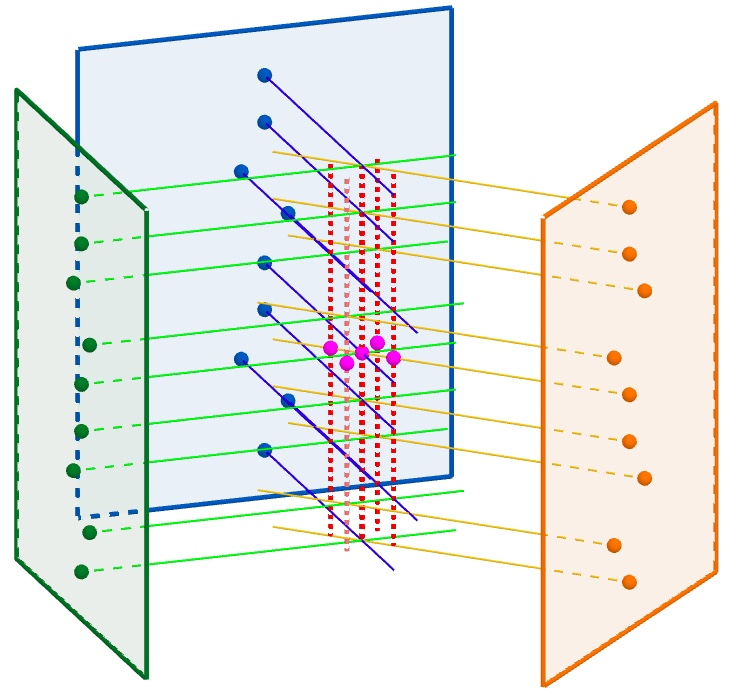
\includegraphics[scale=0.48]{133}

	Рис. 2.6: Изменение точки прямой при фиксированном векторе.
\end{center}

\subsection{Решение}\label{math3:solution}

Пусть имеем три множества:

\begin{center}
	$P_1 = \Set{p_i^1 = (x_i^1, y_i^1, z_i^1)}{i=\ton n_1}$

	\vspace{0.3cm}
	$P_2 = \Set{p_i^2 = (x_i^2, y_i^2, z_i^2)}{i=\ton n_2}$

	\vspace{0.3cm}
	$P_3 = \Set{p_i^3 = (x_i^3, y_i^3, z_i^3)}{i=\ton n_3}$
\end{center}

Также имеем три направления проектирования (векторы нормали плоскостей, которым принадлежат множества $P_1, P_2$ и $P_3$):
$$\begin{gathered}
	r_1 = (r_1^1, r_2^1, r_3^1) \\
	r_2 = (r_1^2, r_2^2, r_3^2) \\
	r_3 = (r_1^3, r_2^3, r_3^3)
\end{gathered}$$

Будем искать прямую в параметрическом виде. Пусть $(m, n, p)$ - напрявляющий вектор прямой, $(x_0, y_0, z_0)$ - некоторая точка прямой. Тогда следующая система задает прямую в $\mathbb{R}^3$: 

\begin{center}
	$\mathit{l}: \; \begin{cases}
		x = x_0 + m \cdot t \\
		y = y_0 + n \cdot t \\
		z = z_0 + p \cdot t
	\end{cases}$, где $t \in \mathbb{R}$ - параметр. 
\end{center}

Проведем через нашу прямую и направления проектирования плоскости:

\begin{center}
	$\pi_1: \; \begin{cases}
		x = x_0 + m \cdot t_1 + r_1^1 \cdot t_2 \\
		y = y_0 + n \cdot t_1 + r_2^1 \cdot t_2 \\
		z = z_0 + p \cdot t_1 + r_3^1 \cdot t_2
	\end{cases}$, где $t_1, t_2 \in \mathbb{R}$ - параметры. 

	\vspace{0.2cm}
	$\pi_2: \; \begin{cases}
		x = x_0 + m \cdot t_1 + r_1^2 \cdot t_2 \\
		y = y_0 + n \cdot t_1 + r_2^2 \cdot t_2 \\
		z = z_0 + p \cdot t_1 + r_3^2 \cdot t_2
	\end{cases}$, где $t_1, t_2 \in \mathbb{R}$ - параметры. 

	\vspace{0.2cm}
	$\pi_3: \; \begin{cases}
		x = x_0 + m \cdot t_1 + r_1^3 \cdot t_2 \\
		y = y_0 + n \cdot t_1 + r_2^3 \cdot t_2 \\
		z = z_0 + p \cdot t_1 + r_3^3 \cdot t_2
	\end{cases}$, где $t_1, t_2 \in \mathbb{R}$ - параметры. 
\end{center}
\newpage
Чтобы найти общие уравнения этих плоскостей, найдем нормали этих плоскостей, которые будем искать как векторное произведение напрявляющих векторов:

$$\begin{gathered}
	n_1 = [l, r_1] = \begin{vmatrix}
		i & j & k \\
		m & n & p \\
		r_1^1 & r_2^1 & r_3^1
	\end{vmatrix} = \left( \begin{vmatrix}
		n & p \\
		r_2^1 & r_3^1
	\end{vmatrix}, -\begin{vmatrix}
		m & p \\
		r_1^1 & r_3^1
	\end{vmatrix}, \begin{vmatrix}
		m & n \\
		r_1^1 & r_2^1
	\end{vmatrix} \right) = \\
	= \left( n r_3^1 - p r_2^1, p r_1^1 - m r_3^1, m r_2^1 - n r_1^1 \right)
\end{gathered}$$
$$\begin{gathered}
	n_2 = [l, r_2] = \begin{vmatrix}
		i & j & k \\
		m & n & p \\
		r_1^2 & r_2^2 & r_3^2
	\end{vmatrix} = \left( \begin{vmatrix}
		n & p \\
		r_2^2 & r_3^2
	\end{vmatrix}, -\begin{vmatrix}
		m & p \\
		r_1^2 & r_3^2
	\end{vmatrix}, \begin{vmatrix}
		m & n \\
		r_1^2 & r_2^2
	\end{vmatrix} \right) = \\
	= \left( n r_3^2 - p r_2^2, p r_1^2 - m r_3^2, m r_2^2 - n r_1^2 \right)
\end{gathered}$$
$$\begin{gathered}
	n_3 = [l, r_3] = \begin{vmatrix}
		i & j & k \\
		m & n & p \\
		r_1^3 & r_2^3 & r_3^3
	\end{vmatrix} = \left( \begin{vmatrix}
		n & p \\
		r_2^3 & r_3^3
	\end{vmatrix}, -\begin{vmatrix}
		m & p \\
		r_1^3 & r_3^3
	\end{vmatrix}, \begin{vmatrix}
		m & n \\
		r_1^3 & r_2^3
	\end{vmatrix} \right) = \\
	= \left( n r_3^3 - p r_2^3, p r_1^3 - m r_3^3, m r_2^3 - n r_1^3 \right)
\end{gathered}$$

Отнормируем векторы нормалей:
$$\begin{gathered}
	(A_1, B_1, C_1) = \frac{\left( n r_3^1 - p r_2^1, p r_1^1 - m r_3^1, m r_2^1 - n r_1^1 \right)}{\sqrt{(n r_3^1 - p r_2^1)^2 + (p r_1^1 - m r_3^1)^2 + (m r_2^1 - n r_1^1)^2}} \\
	(A_2, B_2, C_2) = \frac{\left( n r_3^2 - p r_2^2, p r_1^2 - m r_3^2, m r_2^2 - n r_1^2 \right)}{\sqrt{(n r_3^2 - p r_2^2)^2 + (p r_1^2 - m r_3^2)^2 + (m r_2^2 - n r_1^2)^2}} \\
	(A_3, B_3, C_3) = \frac{\left( n r_3^3 - p r_2^3, p r_1^3 - m r_3^3, m r_2^3 - n r_1^3 \right)}{\sqrt{(n r_3^3 - p r_2^3)^2 + (p r_1^3 - m r_3^3)^2 + (m r_2^3 - n r_1^3)^2}}
\end{gathered}$$

Тогда общие уравнения плоскостей имеют вид:
$$\begin{gathered}
	\pi_1: \; A_1 (x - x_0) + B_1 (y - y_0) + C_1 (z - z_0) = 0 \\
	\pi_2: \; A_2 (x - x_0) + B_2 (y - y_0) + C_2 (z - z_0) = 0 \\
	\pi_3: \; A_3 (x - x_0) + B_3 (y - y_0) + C_3 (z - z_0) = 0 
\end{gathered}$$
Иначе:
$$\begin{gathered}
	\pi_1: \; A_1 x + B_1 y + C_1 z + D_1 = 0 \\
	\pi_2: \; A_2 x + B_2 y + C_2 z + D_2 = 0 \\
	\pi_3: \; A_3 x + B_3 y + C_3 z + D_3 = 0
\end{gathered}$$
$$\begin{gathered}
	\begin{cases}
		A_1 = \frac{n r_3^1 - p r_2^1}{\sqrt{(n r_3^1 - p r_2^1)^2 + (p r_1^1 - m r_3^1)^2 + (m r_2^1 - n r_1^1)^2}} \\
		B_1 = \frac{p r_1^1 - m r_3^1}{\sqrt{(n r_3^1 - p r_2^1)^2 + (p r_1^1 - m r_3^1)^2 + (m r_2^1 - n r_1^1)^2}} \\
		C_1 = \frac{m r_2^1 - n r_1^1}{\sqrt{(n r_3^1 - p r_2^1)^2 + (p r_1^1 - m r_3^1)^2 + (m r_2^1 - n r_1^1)^2}} \\
		D_1 = \frac{- (n r_3^1 - p r_2^1) x_0 - (p r_1^1 - m r_3^1) y_0 - (m r_2^1 - n r_1^1) z_0}{\sqrt{(n r_3^1 - p r_2^1)^2 + (p r_1^1 - m r_3^1)^2 + (m r_2^1 - n r_1^1)^2}}
	\end{cases} \\
	\begin{cases}
		A_2 = \frac{n r_3^2 - p r_2^2}{\sqrt{(n r_3^2 - p r_2^2)^2 + (p r_1^2 - m r_3^2)^2 + (m r_2^2 - n r_1^2)^2}} \\
		B_2 = \frac{p r_1^2 - m r_3^2}{\sqrt{(n r_3^2 - p r_2^2)^2 + (p r_1^2 - m r_3^2)^2 + (m r_2^2 - n r_1^2)^2}} \\
		C_2 = \frac{m r_2^2 - n r_1^2}{\sqrt{(n r_3^2 - p r_2^2)^2 + (p r_1^2 - m r_3^2)^2 + (m r_2^2 - n r_1^2)^2}} \\
		D_2 = \frac{- (n r_3^2 - p r_2^2) x_0 - (p r_1^2 - m r_3^2) y_0 - (m r_2^2 - n r_1^2) z_0}{\sqrt{(n r_3^2 - p r_2^2)^2 + (p r_1^2 - m r_3^2)^2 + (m r_2^2 - n r_1^2)^2}}
	\end{cases} \\
	\begin{cases}
		A_3 = \frac{n r_3^3 - p r_2^3}{\sqrt{(n r_3^3 - p r_2^3)^2 + (p r_1^3 - m r_3^3)^2 + (m r_2^3 - n r_1^3)^2}} \\
		B_3 = \frac{p r_1^3 - m r_3^3}{\sqrt{(n r_3^3 - p r_2^3)^2 + (p r_1^3 - m r_3^3)^2 + (m r_2^3 - n r_1^3)^2}} \\
		C_3 = \frac{m r_2^3 - n r_1^3}{\sqrt{(n r_3^3 - p r_2^3)^2 + (p r_1^3 - m r_3^3)^2 + (m r_2^3 - n r_1^3)^2}} \\
		D_3 = \frac{- (n r_3^3 - p r_2^3) x_0 - (p r_1^3 - m r_3^3) y_0 - (m r_2^3 - n r_1^3) z_0}{\sqrt{(n r_3^3 - p r_2^3)^2 + (p r_1^3 - m r_3^3)^2 + (m r_2^3 - n r_1^3)^2}}
	\end{cases}
\end{gathered}$$

Найдем плоскости, которым принадлежат множества точек:
$$\begin{gathered}
	w_1: \; r_1^1 x + r_2^1 y + r_3^1 z - (r_1^1 x_1^1 + r_2^1 y_1^1 + r_3^1 z_1^1) = 0 \\
	w_2: \; r_1^2 x + r_2^2 y + r_3^2 z - (r_1^2 x_1^2 + r_2^2 y_1^2 + r_3^2 z_1^2) = 0 \\
	w_3: \; r_1^3 x + r_2^3 y + r_3^3 z - (r_1^3 x_1^3 + r_2^3 y_1^3 + r_3^3 z_1^3) = 0
\end{gathered}$$

В пересечении плоскостей $\pi_1$ и $w_1$, $\pi_2$ и $w_2$, $\pi_3$ и $w_3$ получаем проекции исходного отрезка $l_1, l_2, l_3$ на плоскости множеств $w_1, w_2, w_3$. Тогда расстояния от точек множества $P_i$ до проекции $l_i$ на соответствующую плоскость $w_i$ равно расстоянию от этих точек до плоскости $\pi_i$, проходящую через искомый отрезок $l$.

$$\rho (p_i^j, l_j) = |A_j x_i^j + B_j y_i^j + C_j z_i^j + D_j|$$
где $i$ - номер соответствующей точки множества,

$j$ - номер соответствующей плоскости $\pi_j$.\\

Тогда функционал суммы квадратов расстояний от точек множеств до проекций исходного отрезка равен:
$$\Lambda = \underset{j=1}{\overset{3}{\sum}}\underset{i=1}{\overset{n_1, n_2, n_3}{\sum}}(A_j x_i^j + B_j y_i^j + C_j z_i^j + D_j)^2$$
\newpage
Рассмотрим параллельный сдвиг исходного отрезка на некоторый вектор $h$. Будем рассматривать вектор $h$ как вектор, лежащий в плоскости, параллельной OXY, тогда $h = (x_h, y_h, 0)$ и сдвиг будет харакетризоваться этим вектором $h$ полнсотью.\\

Более того, при параллельном переносе исходного отрезка плоскости $\pi_i$ также переносятся параллельно себе, т.е. векторы нормали не изменятся, а изменятся лишь коэффициенты $D_i$ - они умножатся на скалярное произведение вектора $h$ и вектора нормали плоскости $(A_i, B_i, C_i)$. Таким образом, уравнение новых плоскостей $\pi'_j$ будет иметь вид:
$$\begin{gathered}
	A_j x + B_j y + C_j z + D_j \left(h, (A_j, B_j, C_j) \right) = 0 \; \Rightarrow \\
	\Rightarrow \; A_j x + B_j y + C_j z + D_j (x_h A_j + y_h B_j) = 0
\end{gathered}$$

Тогда соответствующий функционал после сдвига имеет вид:
$$\Lambda = \underset{j=1}{\overset{3}{\sum}}\underset{i=1}{\overset{n_1, n_2, n_3}{\sum}}\left(A_j x_i^j + B_j y_i^j + C_j z_i^j + D_j(x_h A_j + y_h B_j)\right)^2$$

Найдем частные производные функционала по $x_h$ и $y_h$:
$$\begin{gathered}
	\begin{cases}
		\frac{\partial}{\partial x_h} \underset{j=1}{\overset{3}{\sum}}\underset{i=1}{\overset{n_1, n_2, n_3}{\sum}}\left(A_j x_i^j + B_j y_i^j + C_j z_i^j + D_j(x_h A_j + y_h B_j)\right)^2 = 0 \\
		\frac{\partial}{\partial y_h} \underset{j=1}{\overset{3}{\sum}}\underset{i=1}{\overset{n_1, n_2, n_3}{\sum}}\left(A_j x_i^j + B_j y_i^j + C_j z_i^j + D_j(x_h A_j + y_h B_j)\right)^2 = 0
	\end{cases} \\
	\begin{cases}
		 \underset{j=1}{\overset{3}{\sum}}\underset{i=1}{\overset{n_1, n_2, n_3}{\sum}}\frac{\partial}{\partial x_h}\left(A_j x_i^j + B_j y_i^j + C_j z_i^j + D_j(x_h A_j + y_h B_j)\right)^2 = 0 \\
		 \underset{j=1}{\overset{3}{\sum}}\underset{i=1}{\overset{n_1, n_2, n_3}{\sum}}\frac{\partial}{\partial y_h}\left(A_j x_i^j + B_j y_i^j + C_j z_i^j + D_j(x_h A_j + y_h B_j)\right)^2 = 0
	\end{cases}\\
	\begin{cases}
		 \underset{j=1}{\overset{3}{\sum}}\underset{i=1}{\overset{n_1, n_2, n_3}{\sum}}\Bigg(2 \left(A_j x_i^j + B_j y_i^j + C_j z_i^j + D_j(x_h A_j + y_h B_j)\right) A_j D_j\Bigg) = 0 \\
		 \underset{j=1}{\overset{3}{\sum}}\underset{i=1}{\overset{n_1, n_2, n_3}{\sum}}\Bigg(2 \left(A_j x_i^j + B_j y_i^j + C_j z_i^j + D_j(x_h A_j + y_h B_j)\right) B_j D_j\Bigg) = 0
	\end{cases}\\
	\begin{cases}
		\underset{j=1}{\overset{3}{\sum}}\underset{i=1}{\overset{n_1, n_2, n_3}{\sum}}\Bigg( A_j^2 D_j^2 x_h + A_j B_j D_j^2 y_h + A_j D_j \left(  A_j x_i^j + B_j y_i^j + C_j z_i^j\right) \Bigg) = 0 \\
		\underset{j=1}{\overset{3}{\sum}}\underset{i=1}{\overset{n_1, n_2, n_3}{\sum}}\Bigg( A_j B_j D_j^2 x_h + B_j^2 D_j^2 y_h + B_j D_j \left( A_j x_i^j + B_j y_i^j + C_j z_i^j \right) \Bigg) = 0
	\end{cases}
\end{gathered}$$
\newpage
Получаем линейную систему на $x_h, y_h$:
$$\begin{cases}
	\Bigg( \underset{j=1}{\overset{3}{\sum}}\underset{i=1}{\overset{n_1, n_2, n_3}{\sum}} A_j^2 D_j^2 \Bigg) x_h + \Bigg( \underset{j=1}{\overset{3}{\sum}}\underset{i=1}{\overset{n_1, n_2, n_3}{\sum}} A_j B_j D_j^2 \Bigg) y_h + \\
	\hspace{1cm} + \Bigg( \underset{j=1}{\overset{3}{\sum}}\underset{i=1}{\overset{n_1, n_2, n_3}{\sum}} A_j D_j \left(  A_j x_i^j + B_j y_i^j + C_j z_i^j\right) \Bigg) = 0 \\
	\Bigg( \underset{j=1}{\overset{3}{\sum}}\underset{i=1}{\overset{n_1, n_2, n_3}{\sum}} A_j B_j D_j^2 \Bigg) x_h + \Bigg( \underset{j=1}{\overset{3}{\sum}}\underset{i=1}{\overset{n_1, n_2, n_3}{\sum}} B_j^2 D_j^2 \Bigg) y_h + \\
	\hspace{1cm} + \Bigg( \underset{j=1}{\overset{3}{\sum}}\underset{i=1}{\overset{n_1, n_2, n_3}{\sum}} B_j D_j \left( A_j x_i^j + B_j y_i^j + C_j z_i^j \right) \Bigg) = 0
\end{cases}$$
Введем обозначения:
$$\begin{cases}
	a_{11} = \underset{j=1}{\overset{3}{\sum}}\underset{i=1}{\overset{n_1, n_2, n_3}{\sum}} A_j^2 D_j^2 \\
	a_{12} = a_{21} = \underset{j=1}{\overset{3}{\sum}}\underset{i=1}{\overset{n_1, n_2, n_3}{\sum}} A_j B_j D_j^2 \\
	a_{22} = \underset{j=1}{\overset{3}{\sum}}\underset{i=1}{\overset{n_1, n_2, n_3}{\sum}} B_j^2 D_j^2 \\
	b_1 = \underset{j=1}{\overset{3}{\sum}}\underset{i=1}{\overset{n_1, n_2, n_3}{\sum}} A_j D_j \left(  A_j x_i^j + B_j y_i^j + C_j z_i^j\right) \\
	b_2 = \underset{j=1}{\overset{3}{\sum}}\underset{i=1}{\overset{n_1, n_2, n_3}{\sum}} B_j D_j \left( A_j x_i^j + B_j y_i^j + C_j z_i^j \right)
\end{cases}$$
Если система невырождена, то получаем решение:
$$\begin{cases}
	x_h = \frac{a_{22} b_1 - a_{12} b_2}{a_{12}^2 - a_{11}a_{22}} \\
	y_h = \frac{a_{11} b_2 - a_{12} b_1}{a_{12}^2 - a_{11}a_{22}}
\end{cases}$$

\vspace{0.5cm}
Теперь будем рассматривать поворот исходного отрезка вокруг точки $(x_0, y_0, z_0)$ - середины отрезка. Пусть один конец переместили на вектор $h = (x_h, y_h, 0)$, тогда новое уравнение прямой имеет вид:

\begin{center}
	$\mathit{l}: \; \begin{cases}
		x = x_0 + (m + x_h) \cdot t \\
		y = y_0 + (n + y_h) \cdot t \\
		z = z_0 + p \cdot t
	\end{cases}$, где $t \in \mathbb{R}$ - параметр. 
\end{center}

Тогда уравнения плоскостей, проходящие через повернутую прямую имеют вид:
$$\begin{gathered}
	\pi_1: \; A_1 x + B_1 y + C_1 z + D_1 = 0 \\
	\pi_2: \; A_2 x + B_2 y + C_2 z + D_2 = 0 \\
	\pi_3: \; A_3 x + B_3 y + C_3 z + D_3 = 0
\end{gathered}$$
$$\begin{gathered}
	\begin{cases}
		A_1 = \frac{(n + y_h) r_3^1 - p r_2^1}{\sqrt{((n + y_h) r_3^1 - p r_2^1)^2 + (p r_1^1 - (m + x_h) r_3^1)^2 + ((m + x_h) r_2^1 - (n + y_h) r_1^1)^2}} \\
		B_1 = \frac{p r_1^1 - (m + x_h) r_3^1}{\sqrt{((n + y_h) r_3^1 - p r_2^1)^2 + (p r_1^1 - (m + x_h) r_3^1)^2 + ((m + x_h) r_2^1 - (n + y_h) r_1^1)^2}} \\
		C_1 = \frac{(m + x_h) r_2^1 - (n + y_h) r_1^1}{\sqrt{((n + y_h) r_3^1 - p r_2^1)^2 + (p r_1^1 - (m + x_h) r_3^1)^2 + ((m + x_h) r_2^1 - (n + y_h) r_1^1)^2}} \\
		D_1 = \frac{- ((n + y_h) r_3^1 - p r_2^1) x_0 - (p r_1^1 - (m + x_h) r_3^1) y_0 - ((m + x_h) r_2^1 - (n + y_h) r_1^1) z_0}{\sqrt{((n + y_h) r_3^1 - p r_2^1)^2 + (p r_1^1 - (m + x_h) r_3^1)^2 + ((m + x_h) r_2^1 - (n + y_h) r_1^1)^2}}
	\end{cases} \\
	\begin{cases}
		A_2 = \frac{(n + y_h) r_3^2 - p r_2^2}{\sqrt{((n + y_h) r_3^2 - p r_2^2)^2 + (p r_1^2 - (m + x_h) r_3^2)^2 + ((m + x_h) r_2^2 - (n + y_h) r_1^2)^2}} \\
		B_2 = \frac{p r_1^2 - (m + x_h) r_3^2}{\sqrt{((n + y_h) r_3^2 - p r_2^2)^2 + (p r_1^2 - (m + x_h) r_3^2)^2 + ((m + x_h) r_2^2 - (n + y_h) r_1^2)^2}} \\
		C_2 = \frac{(m + x_h) r_2^2 - (n + y_h) r_1^2}{\sqrt{((n + y_h) r_3^2 - p r_2^2)^2 + (p r_1^2 - (m + x_h) r_3^2)^2 + ((m + x_h) r_2^2 - (n + y_h) r_1^2)^2}} \\
		D_2 = \frac{- ((n + y_h) r_3^2 - p r_2^2) x_0 - (p r_1^2 - (m + x_h) r_3^2) y_0 - ((m + x_h) r_2^2 - (n + y_h) r_1^2) z_0}{\sqrt{((n + y_h) r_3^2 - p r_2^2)^2 + (p r_1^2 - (m + x_h) r_3^2)^2 + ((m + x_h) r_2^2 - (n + y_h) r_1^2)^2}}
	\end{cases} \\
	\begin{cases}
		A_3 = \frac{(n + y_h) r_3^3 - p r_2^3}{\sqrt{((n + y_h) r_3^3 - p r_2^3)^2 + (p r_1^3 - (m + x_h) r_3^3)^2 + ((m + x_h) r_2^3 - (n + y_h) r_1^3)^2}} \\
		B_3 = \frac{p r_1^3 - (m + x_h) r_3^3}{\sqrt{((n + y_h) r_3^3 - p r_2^3)^2 + (p r_1^3 - (m + x_h) r_3^3)^2 + ((m + x_h) r_2^3 - (n + y_h) r_1^3)^2}} \\
		C_3 = \frac{(m + x_h) r_2^3 - (n + y_h) r_1^3}{\sqrt{((n + y_h) r_3^3 - p r_2^3)^2 + (p r_1^3 - (m + x_h) r_3^3)^2 + ((m + x_h) r_2^3 - (n + y_h) r_1^3)^2}} \\
		D_3 = \frac{- ((n + y_h) r_3^3 - p r_2^3) x_0 - (p r_1^3 - (m + x_h) r_3^3) y_0 - ((m + x_h) r_2^3 - (n + y_h) r_1^3) z_0}{\sqrt{((n + y_h) r_3^3 - p r_2^3)^2 + (p r_1^3 - (m + x_h) r_3^3)^2 + ((m + x_h) r_2^3 - (n + y_h) r_1^3)^2}}
	\end{cases}
\end{gathered}$$

\vspace{1cm}
Вместо выражения исходного функционала суммы квадратов расстояний рассмотрим лишь числитель функционала, получаем следующий функционал для каждого из множеств:
$$\begin{gathered}
	\Lambda' = \underset{i=1}{\overset{n_j}{\sum}} \Bigg( \left( (n+y_h)r_3^j - p r_2^j \right)x_i^j + \left( p r_1^j - (m+x_h) r_3^j \right)y_i^j + \\ 
	\hspace{0.5cm} + \left( (m+x_h)r_2^j - (n+y_h)r_1^j \right) z_i^j - ((n + y_h) r_3^j - p r_2^j) x_0 -  \\
	\hspace{1cm} - (p r_1^j - (m + x_h) r_3^j) y_0 - ((m + x_h) r_2^j - (n + y_h) r_1^j) z_0 \Bigg)^2 \\
	j = 1,2,3
\end{gathered}$$

Мы не можем суммировать все суммы квадратов, т.к. для разных плоскостей разные выражения в знаменателе, и избавиться от всех них при подсчете не получится.\\

Чтобы получить единственный оптимальный поворот для всех плоскостей решим проблему знаменателей следующим образом. При итерации поворота в знаменатели подставим значения $x_h$ и $y_h$ предыдущей итерации, на начальном шаге возьмем нулевые $x_h$ и $y_h$. Таким образом мы будем рассматривать сумму значений функционалов для плоскостей с некоторыми весами, равными обратным значениям знаменателей с подставновкой, описанной выше. Эту сумму и необходимо будет минимизировать по $x_h$ и $y_h$. Новый функционал имеет вид:
$$\begin{gathered}
	\Lambda' = \underset{i=1}{\overset{3}{\sum}}w_{i-1}\underset{j=1}{\overset{n_i}{\sum}} \Bigg( \left( (n+y_h)r_3^j - p r_2^j \right)x_i^j + \left( p r_1^j - (m+x_h) r_3^j \right)y_i^j + \\ 
	\hspace{0.5cm} + \left( (m+x_h)r_2^j - (n+y_h)r_1^j \right) z_i^j - ((n + y_h) r_3^j - p r_2^j) x_0 -  \\
	\hspace{1cm} - (p r_1^j - (m + x_h) r_3^j) y_0 - ((m + x_h) r_2^j - (n + y_h) r_1^j) z_0 \Bigg)^2 \\
	j = 1,2,3, \;\; w_{i-1} \text{ - значение знаменателя при } x_h, y_h \text{ из предыдущей итерации}
\end{gathered}$$
Найдем частные производные функционала по $x_h$ и $y_h$:
$$\begin{gathered}
	\begin{cases}
		\frac{\partial}{\partial x_h} \underset{i=1}{\overset{3}{\sum}}w_{i-1}\underset{j=1}{\overset{n_i}{\sum}} \Bigg( \left( (n+y_h)r_3^j - p r_2^j \right)x_i^j + \left( p r_1^j - (m+x_h) r_3^j \right)y_i^j + \\
		\hspace{1.5cm} + \left( (m+x_h)r_2^j - (n+y_h)r_1^j \right) z_i^j - ((n + y_h) r_3^j - p r_2^j) x_0 - \\
		\hspace{1.5cm} - (p r_1^j - (m + x_h) r_3^j) y_0 - ((m + x_h) r_2^j - (n + y_h) r_1^j) z_0 \Bigg)^2 = 0 \\
		\frac{\partial}{\partial y_h} \underset{i=1}{\overset{3}{\sum}}w_{i-1}\underset{j=1}{\overset{n_i}{\sum}} \Bigg( \left( (n+y_h)r_3^j - p r_2^j \right)x_i^j + \left( p r_1^j - (m+x_h) r_3^j \right)y_i^j + \\
		\hspace{1.5cm} + \left( (m+x_h)r_2^j - (n+y_h)r_1^j \right) z_i^j - ((n + y_h) r_3^j - p r_2^j) x_0 - \\
		\hspace{1.5cm} - (p r_1^j - (m + x_h) r_3^j) y_0 - ((m + x_h) r_2^j - (n + y_h) r_1^j) z_0 \Bigg)^2 = 0
	\end{cases}
\end{gathered}$$
$$\begin{gathered}
	\begin{cases}
		 \underset{i=1}{\overset{3}{\sum}}w_{i-1}\underset{j=1}{\overset{n_i}{\sum}} \frac{\partial}{\partial x_h} \Bigg( \left( (n+y_h)r_3^j - p r_2^j \right)x_i^j + \left( p r_1^j - (m+x_h) r_3^j \right)y_i^j + \\
		\hspace{1.5cm} + \left( (m+x_h)r_2^j - (n+y_h)r_1^j \right) z_i^j - ((n + y_h) r_3^j - p r_2^j) x_0 - \\
		\hspace{1.5cm} - (p r_1^j - (m + x_h) r_3^j) y_0 - ((m + x_h) r_2^j - (n + y_h) r_1^j) z_0 \Bigg)^2 = 0 \\
		\underset{i=1}{\overset{3}{\sum}}w_{i-1}\underset{j=1}{\overset{n_i}{\sum}} \frac{\partial}{\partial y_h} \Bigg( \left( (n+y_h)r_3^j - p r_2^j \right)x_i^j + \left( p r_1^j - (m+x_h) r_3^j \right)y_i^j + \\
		\hspace{1.5cm} + \left( (m+x_h)r_2^j - (n+y_h)r_1^j \right) z_i^j - ((n + y_h) r_3^j - p r_2^j) x_0 - \\
		\hspace{1.5cm} - (p r_1^j - (m + x_h) r_3^j) y_0 - ((m + x_h) r_2^j - (n + y_h) r_1^j) z_0 \Bigg)^2 = 0
	\end{cases}
\end{gathered}$$
$$\begin{gathered}
	\begin{cases}
		\underset{i=1}{\overset{3}{\sum}}w_{i-1}\underset{j=1}{\overset{n_i}{\sum}} \Bigg( \left( (n+y_h)r_3^j - p r_2^j \right)x_i^j + \left( p r_1^j - (m+x_h) r_3^j \right)y_i^j + \\
		\hspace{1.5cm} + \left( (m+x_h)r_2^j - (n+y_h)r_1^j \right) z_i^j - ((n + y_h) r_3^j - p r_2^j) x_0 - \\
		\hspace{1.5cm} - (p r_1^j - (m + x_h) r_3^j) y_0 - ((m + x_h) r_2^j - (n + y_h) r_1^j) z_0 \Bigg) \times \\
		\hspace{1.5cm} \times \Bigg( - r_3^j y_i^j + r_2^j z_i^j + r_3^j y_0 - r_2^j z_0 \Bigg) = 0 \\
		\underset{i=1}{\overset{3}{\sum}}w_{i-1}\underset{j=1}{\overset{n_i}{\sum}} \Bigg( \left( (n+y_h)r_3^j - p r_2^j \right)x_i^j + \left( p r_1^j - (m+x_h) r_3^j \right)y_i^j + \\
		\hspace{1.5cm} + \left( (m+x_h)r_2^j - (n+y_h)r_1^j \right) z_i^j - ((n + y_h) r_3^j - p r_2^j) x_0 - \\
		\hspace{1.5cm} - (p r_1^j - (m + x_h) r_3^j) y_0 - ((m + x_h) r_2^j - (n + y_h) r_1^j) z_0 \Bigg) \times \\
		\hspace{1.5cm} \times \Bigg( r_3^j x_i^j - r_1^j z_i^j - r_3^j x_0 + r_1^j z_0 \Bigg) = 0 
	\end{cases}
\end{gathered}$$

$$\begin{gathered}
	\begin{cases}
		\underset{i=1}{\overset{3}{\sum}}w_{i-1}\underset{j=1}{\overset{n_i}{\sum}}
		\left( -r_3^j y_i^j + r_2^j z_i^j + r_3^j y_0 -r_2^j z_0 \right) 
		\left( - r_3^j y_i^j + r_2^j z_i^j + r_3^j y_0 - r_2^j z_0 \right) 
		x_h + \\
		\hspace{1cm} + \underset{i=1}{\overset{3}{\sum}}w_{i-1}\underset{j=1}{\overset{n_i}{\sum}}
		\left( r_3^j x_i^j - r_1^j z_i^j - r_3^j x_0 + r_1^j z_0 \right) 
		\left( - r_3^j y_i^j + r_2^j z_i^j + r_3^j y_0 - r_2^j z_0 \right) 
		y_h + \\
		\hspace{1cm} + \underset{i=1}{\overset{3}{\sum}}w_{i-1}\underset{j=1}{\overset{n_i}{\sum}}
		\Bigg( \left( n r_3^j - p r_2^j \right)x_i^j + \left( p r_1^j - m r_3^j \right)y_i^j + \left( m r_2^j - n r_1^j \right) z_i^j -  \\
		\hspace{1.5cm} - (n r_3^j - p r_2^j) x_0 - (p r_1^j - m r_3^j) y_0 - (m r_2^j - n r_1^j) z_0 \Bigg) \times \\
		\hspace{1cm} \times \left( - r_3^j y_i^j + r_2^j z_i^j + r_3^j y_0 - r_2^j z_0 \right) = 0 \\ \\
		\underset{i=1}{\overset{3}{\sum}}w_{i-1}\underset{j=1}{\overset{n_i}{\sum}}
		\left( -r_3^j y_i^j + r_2^j z_i^j + r_3^j y_0 - r_2^j z_0 \right) 
		\left( r_3^j x_i^j - r_1^j z_i^j - r_3^j x_0 + r_1^j z_0 \right) 
		x_h + \\
		\hspace{1cm} + \underset{i=1}{\overset{3}{\sum}}w_{i-1}\underset{j=1}{\overset{n_i}{\sum}}
		\left( r_3^j x_i^j - r_1^j z_i^j - r_3^j x_0 + r_1^j z_0 \right) 
		\left( r_3^j x_i^j - r_1^j z_i^j - r_3^j x_0 + r_1^j z_0 \right) 
		y_h + \\
		\hspace{1cm} + \underset{i=1}{\overset{3}{\sum}}w_{i-1}\underset{j=1}{\overset{n_i}{\sum}}
		\Bigg( \left( n r_3^j - p r_2^j \right)x_i^j + \left( p r_1^j - m r_3^j \right)y_i^j + \left( m r_2^j - n r_1^j \right) z_i^j -  \\
		\hspace{1.5cm} - (n r_3^j - p r_2^j) x_0 - (p r_1^j - m r_3^j) y_0 - (m r_2^j - n r_1^j) z_0 \Bigg) \times \\
		\hspace{1cm} \times \left( r_3^j x_i^j - r_1^j z_i^j - r_3^j x_0 + r_1^j z_0 \right) = 0
	\end{cases}
\end{gathered}$$

\newpage
Введем обозначения:
$$\begin{cases}
	a_{11} = \underset{i=1}{\overset{3}{\sum}}w_{i-1}\underset{j=1}{\overset{n_i}{\sum}} 
		\left( -r_3^j y_i^j + r_2^j z_i^j + r_3^j y_0 -r_2^j z_0 \right)^2 \\
	a_{12} = a_{21} = \underset{i=1}{\overset{3}{\sum}}w_{i-1}\underset{j=1}{\overset{n_i}{\sum}}
		\left( r_3^j x_i^j - r_1^j z_i^j - r_3^j x_0 + r_1^j z_0 \right) \left( - r_3^j y_i^j + r_2^j z_i^j + r_3^j y_0 - r_2^j z_0 \right) \\
	a_{22} = \underset{i=1}{\overset{3}{\sum}}w_{i-1}\underset{j=1}{\overset{n_i}{\sum}}
		\left( r_3^j x_i^j - r_1^j z_i^j - r_3^j x_0 + r_1^j z_0 \right)^2\\
	b_1 = \underset{i=1}{\overset{3}{\sum}}w_{i-1}\underset{j=1}{\overset{n_i}{\sum}}
		\Bigg( \left( n r_3^j - p r_2^j \right)x_i^j + \left( p r_1^j - m r_3^j \right)y_i^j + \left( m r_2^j - n r_1^j \right) z_i^j -  \\
		\hspace{1.5cm} - (n r_3^j - p r_2^j) x_0 - (p r_1^j - m r_3^j) y_0 - (m r_2^j - n r_1^j) z_0 \Bigg) \times \\
		\hspace{1cm} \times \left( - r_3^j y_i^j + r_2^j z_i^j + r_3^j y_0 - r_2^j z_0 \right) \\
	b_2 = \underset{i=1}{\overset{3}{\sum}}w_{i-1}\underset{j=1}{\overset{n_i}{\sum}}
		\Bigg( \left( n r_3^j - p r_2^j \right)x_i^j + \left( p r_1^j - m r_3^j \right)y_i^j + \left( m r_2^j - n r_1^j \right) z_i^j -  \\
		\hspace{1.5cm} - (n r_3^j - p r_2^j) x_0 - (p r_1^j - m r_3^j) y_0 - (m r_2^j - n r_1^j) z_0 \Bigg) \times \\
		\hspace{1cm} \times \left( r_3^j x_i^j - r_1^j z_i^j - r_3^j x_0 + r_1^j z_0 \right)
\end{cases}$$
Если система невырождена, то получаем решение:
$$\begin{cases}
	x_h = \frac{a_{22} b_1 - a_{12} b_2}{a_{12}^2 - a_{11}a_{22}} \\
	y_h = \frac{a_{11} b_2 - a_{12} b_1}{a_{12}^2 - a_{11}a_{22}}
\end{cases}$$

Таким образом, находим вектор $h$, которые минимизирует функционал поворота для всех плоскостей.\\

Поочередное применения параллельного переноса и поворота приводит прямую в искомое положение. 

\subsection{Погрешность и примеры работы программ}\label{math3:error}

Погрешность метода складывается из погрешности выбора начального положения прямой, а также из погрешностей методов параллельного переноса и поворота.

\newpage
\subsubsection{Искусственные данные}\label{math2:error:synth}

Исходные данные - три множетсва точек и три направления проектирования:

\begin{verbatim}
	(2, -4, 0)	          (-4, 2, 0)            (6.242641, 6.242641, 0)
	(2.1, -4, 1)         (-4, 2.1, 1)          (6.342641, 6.142641, 1)
	(1.9, -4, 2)         (-4, 1.9, 2)          (6.242641, 6.242641, 1.5)
	(2, -4, 3)           (-4, 2, 3)            (6.142641, 6.342641, 2)
	(2, -4, 4)           (-4, 2, 4)            (6.242641, 6.242641, 3)
	(2.1, -4, 5)         (-4, 2.1, 5)          (6.242641, 6.242641, 4)
	(1.9, -4, 6)         (-4, 1.9, 6)          (6.342641, 6.142641, 5)
	(2, -4, 7)           (-4, 2, 6.5)          (6.142641, 6.342641, 6)
	(2, -4, 7.5)         (-4, 2, 7)            (6.242641, 6.242641, 7)
	(2, -4, 8)           (-4, 2, 8)            (6.242641, 6.242641, 8)

	(0, 1, 0)            (1, 0, 0)             (-0.707107, -0.707107, 0)
\end{verbatim}

Полученные данные - направляющий вектор прямой, точка прямой и значение функционала:

\subsubsection{Реальные данные}\label{math2:error:real}

Исходные данные - 100 множетсв точек и 100 направлений проектирования отрезка, ограниченного по $z$ значениями $-6.08332812434530$ и $-4.57712089734895$. Фигура симметричная, поэтому имеем два искомых отрезка.\\

Полученные данные - по две точки искомых прямых и значения функционала:

\newpage


